% ============================================================
%  CISTOGRAFÍA / CISTOURETROGRAFÍA
%  Licenciatura en Imagenología --- UdelaR
%  Imagenología Especializada I, 2026
%  Lic. Camila Mier
%
%  IMPORTANTE: Este archivo NO tiene \documentclass ni
%  \begin{document}. Todo eso vive en main.tex.
%  Compila siempre desde main.tex con XeLaTeX.
% ============================================================

\chapter{Cistografia}



% ============================================================
%  PUNTOS CLAVE PARA EL EXAMEN ORAL
% ============================================================
\begin{cajakeypoints}
\textbf{\color{azulprincipal} Puntos clave para el examen oral}
\begin{itemize}[noitemsep, topsep=2pt]
  \item Es una exploración radiológica del \textbf{tracto urinario inferior}: vejiga y uretra.
  \item La uretra femenina mide \textbf{4 cm}; la masculina varía entre \textbf{17,5 y 20 cm} (anterior: peneana + bulbar; posterior: prostática + membranosa).
  \item Se requiere \textbf{urocultivo negativo 72 horas antes} del estudio.
  \item Contraindicaciones absolutas: \textbf{infección aguda}, obstrucción uretral completa y embarazo.
  \item Sonda Foley: calibre \textbf{12--18 F} en adultos, \textbf{5--8 F} en niños. En el hombre se fija en la \textbf{fosa navicular} inflando el balón con \textbf{1--1,5 mL} de solución salina.
  \item Volumen de contraste yodado hidrosoluble: \textbf{400--450 mL}.
  \item Residuo post-miccional \textbf{mayor al 30\%} del volumen inicial se considera anormal.
  \item La estenosis de uretra anterior se valora en \textbf{fase de llenado}; la de uretra posterior en \textbf{proyecciones transmiccionales}.
\end{itemize}
\end{cajakeypoints}

\vspace{1em}

% ============================================================
%  SECCIÓN 1 --- DEFINICIÓN
% ============================================================
\section*{Definición}

\begin{cajadefinicion}
La \textbf{cistografía} (o cistouretrografía) es una exploración radiológica del tracto urinario inferior que permite estudiar la vejiga y la uretra mediante instilación retrógrada de contraste yodado hidrosoluble a través de una sonda vesical.
\end{cajadefinicion}

El estudio se practica preferentemente en varones para estudiar la totalidad de la uretra, aunque también se realiza en mujeres. Continúa siendo el \textbf{método diagnóstico inicial} para muchas enfermedades del sistema urinario inferior debido a su fácil acceso, bajo costo y gran exactitud.

% ============================================================
%  SECCIÓN 2 --- ANATOMÍA DE REFERENCIA
% ============================================================
\section*{Anatomía de Referencia}

\subsection*{Uretra femenina}

La uretra femenina mide aproximadamente \textbf{4 cm} de largo y se extiende desde el cuello de la vejiga en la unión ureterovesical hasta el vestíbulo, donde forma el meato externo entre los labios menores.

\subsection*{Uretra masculina}

La uretra masculina varía de \textbf{17,5 a 20 cm} de longitud y se divide en dos segmentos principales:

{\renewcommand{\arraystretch}{1.35}
\begin{center}
\begin{tabular}{>{\bfseries}p{3cm} p{4cm} p{6.5cm}}
\hline
Segmento & División & Porción \\
\hline
Posterior & Preprostática & Cuello vesical hasta próstata. \\[0.3em]
\hline
          & Prostática     & Atraviesa la próstata. \\[0.3em]
\hline
          & Membranosa     & Porción más corta; atraviesa el diafragma urogenital. \\[0.5em]
\hline
Anterior  & Bulbar         & Desde la membrana perineal hasta el pene. \\[0.3em]
\hline
          & Peneana        & Recorre el cuerpo del pene hasta la fosa navicular. \\
\hline
\end{tabular}
\end{center} 
}

% ============================================================
%  SECCIÓN 3 --- INDICACIONES
% ============================================================
\section*{Indicaciones}

\subsection*{Patológicas}

\begin{itemize}[noitemsep]
  \item Valoración de \textbf{estenosis}, estrecheces, traumatismos y tumores.
  \item \textbf{Reflujo vesicoureteral}.
  \item Infecciones urinarias recurrentes.
  \item Trastornos neurogénicos.
  \item Anomalías anatómicas.
  \item \textbf{Divertículos vesicales} (más frecuentes en la mujer).
  \item Incontinencia urinaria.
  \item Fístulas desde el aparato urinario al genital, digestivo o a la piel.
  \item Defecto de llenado.
  \item Hematuria.
\end{itemize}

% ============================================================
%  SECCIÓN 4 --- PREPARACIÓN Y CONTRAINDICACIONES
% ============================================================
\section*{Preparación Previa y Contraindicaciones}

\subsection*{Preparación previa}

El estudio \textbf{no requiere ayuno ni preparación intestinal}. Los pasos previos obligatorios son:

\begin{enumerate}[noitemsep]
  \item Realizar \textbf{urocultivo 72 horas antes}; el resultado debe ser negativo.
  \item Interrogar al paciente sobre \textbf{alergias} a medios de contraste, medicamentos o alimentos.
  \item Obtener \textbf{consentimiento informado} firmado.
\end{enumerate}

\clearpage

\subsection*{Contraindicaciones}

\begin{cajariesgo}
\textbf{Contraindicaciones absolutas:}
\begin{itemize}[noitemsep, topsep=2pt]
  \item Infección en período agudo (el urocultivo positivo es criterio de exclusión).
  \item Obstrucción uretral completa.
  \item Embarazo.
\end{itemize}
\end{cajariesgo}

% ============================================================
%  SECCIÓN 5 --- PROTOCOLO DE PROCEDIMIENTO
% ============================================================
\section*{Protocolo de Procedimiento}

\subsection*{Posición del paciente y preparación}

El paciente debe \textbf{orinar} antes de comenzar el estudio para vaciar la vejiga. A continuación se posiciona en \textbf{decúbito supino} sobre la mesa radiográfica.

\subsection*{Sondaje vesical}

\begin{enumerate}[noitemsep]
  \item Limpieza de genitales con \textbf{antiséptico}.
  \item Aplicación de \textbf{xilocaína en gel al 2\%} (anestésico local) en el meato uretral.
  \item Introducción de \textbf{sonda Foley}: calibre \textbf{12--18 F} en adultos y \textbf{5--8 F} en niños.
  \item \textbf{Fijación de la sonda:}
    \begin{itemize}[noitemsep]
      \item \textit{Hombres:} se fija a la altura de la \textbf{fosa navicular} inflando el balón con \textbf{1--1,5 mL} de solución salina.
      \item \textit{Mujeres:} se introduce hasta la luz de la vejiga y se fija directamente.
    \end{itemize}
  \item Instilación de \textbf{contraste yodado hidrosoluble} a través de la sonda, hasta un volumen de \textbf{400--450 mL}, hasta llenar la vejiga.
\end{enumerate}

\clearpage
% ============================================================
%  SECCIÓN 6 --- PROYECCIONES RADIOLÓGICAS
% ============================================================
\section*{Proyecciones Radiológicas}

Las proyecciones se realizan en el siguiente orden secuencial:

{\renewcommand{\arraystretch}{1.35}
\begin{center}
\begin{tabular}{>{\bfseries}p{3.5cm} p{4.5cm} p{5.5cm}}
\hline
Proyección & Momento & Lo que se evalúa \\
\hline
Aparato urinario simple & Previo al contraste & Cuerpos extraños, calcificaciones, alteraciones óseas. \\[0.5em]
\hline
Uretra & Fase de llenado & Anatomía uretral; estenosis de uretra anterior. \\[0.5em]
\hline
AP de pelvis (llenado parcial) & Durante el llenado & Ureteroceles y tumores (que podrían no verse con vejiga llena). \\[0.5em]
\hline
AP de pelvis (vejiga llena) supino y de pie & Vejiga llena & Morfología vesical, paredes, defectos de llenado, capacidad, descenso del piso; reflujo vesicoureteral en mujeres (fluoroscopia). \\[0.5em]
\hline
Oblicuas a 45° & Durante la micción & Unión vesicoureteral en busca de reflujo; márgenes vesicales. \\[0.5em]
\hline
Lateral & Durante la micción & Ángulos uretrales, descenso vesical; indicada en sospecha de incontinencia urinaria o fístulas (principalmente en mujeres). \\[0.5em]
\hline
Post-miccional & Tras la micción & Verificación de eliminación del contraste; residuo $>$30\% es anormal. Fluoroscopia de riñones para descartar reflujo. \\
\hline
\end{tabular}
\end{center}
}

\begin{figure}[h]
    \centering
    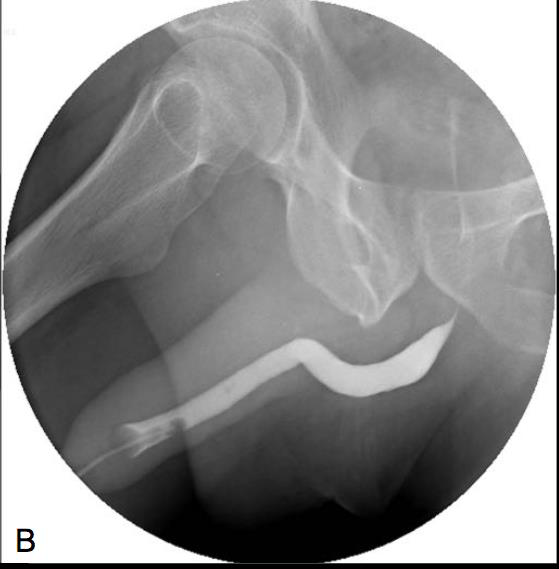
\includegraphics[width=0.5\linewidth]{imagenes/cisto1.png}
    \caption{Uretra durante llenado}
    \label{fig:c1}
\end{figure}

\begin{figure}
    \centering
    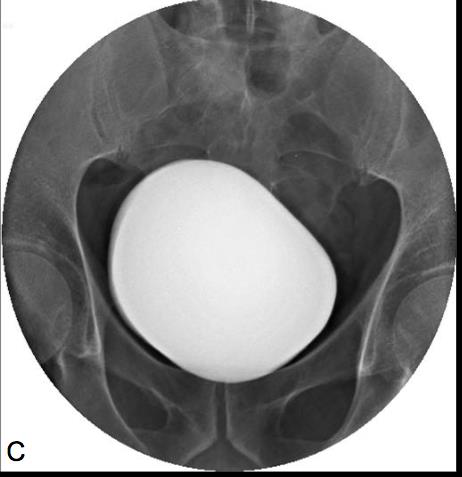
\includegraphics[width=0.5\linewidth]{imagenes/Cisto 2.png}
    \caption{Vejiga llena}
    \label{fig:c2}
\end{figure}

\begin{figure}
    \centering
    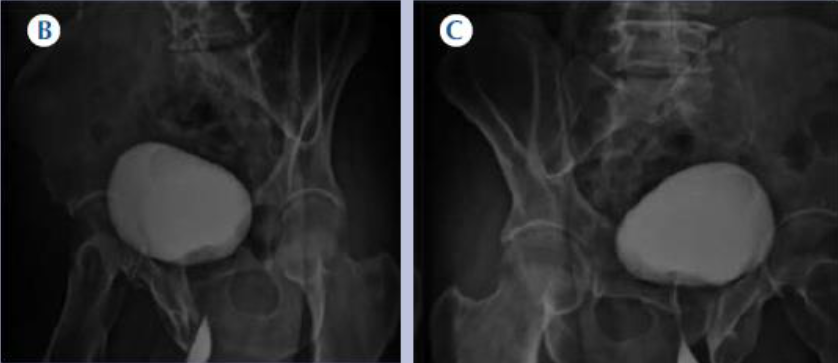
\includegraphics[width=1\linewidth]{imagenes/cisto4.png}
    \caption{Oblicuas, B derecha, C izquierda}
    \label{fig:c3}
\end{figure}

\begin{figure}
    \centering
    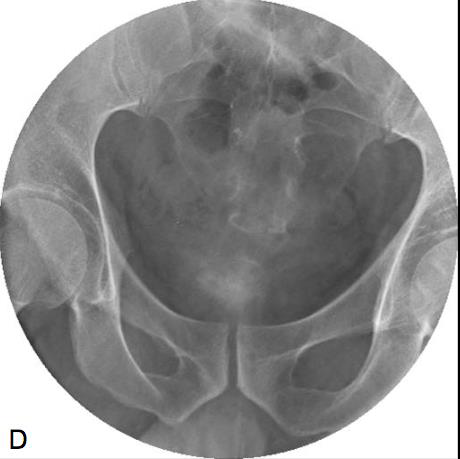
\includegraphics[width=0.5\linewidth]{imagenes/cisto5.png}
    \caption{Post micción}
    \label{fig:c4}
\end{figure}

\clearpage
% ============================================================
%  SECCIÓN 7 --- HALLAZGOS PATOLÓGICOS
% ============================================================
\section*{Hallazgos Patológicos Principales}

\subsection*{Estenosis uretral}

La estenosis restringe el flujo de orina desde la vejiga y puede generar inflamación o infección del tracto urinario. Es más frecuente en los \textbf{hombres} debido a la mayor longitud de la uretra.\\


\begin{cajakeypoints}
\textbf{Regla de valoración:} Uretra anterior $\to$ fase de \textbf{llenado}. \quad Uretra posterior $\to$ proyecciones \textbf{transmiccionales}.
\end{cajakeypoints}

\begin{figure}[h]
    \centering
    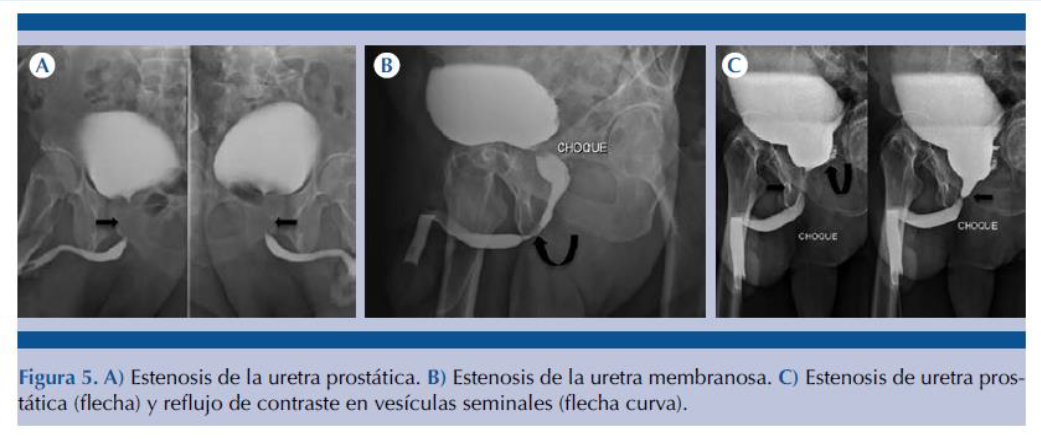
\includegraphics[width=1\linewidth]{imagenes/cisto estenosis.png}
    \caption{Estenosis}
    \label{fig:placeholder}
\end{figure}

\subsection*{Reflujo vesicoureteral}

Flujo anormal de orina que asciende de forma retrógrada desde la vejiga hacia el sistema urinario superior. Puede desencadenar infecciones urinarias recurrentes y, en su evolución, \textbf{falla renal}. Se detecta con fluoroscopia durante el llenado y la micción.

\begin{figure}[h]
    \centering
    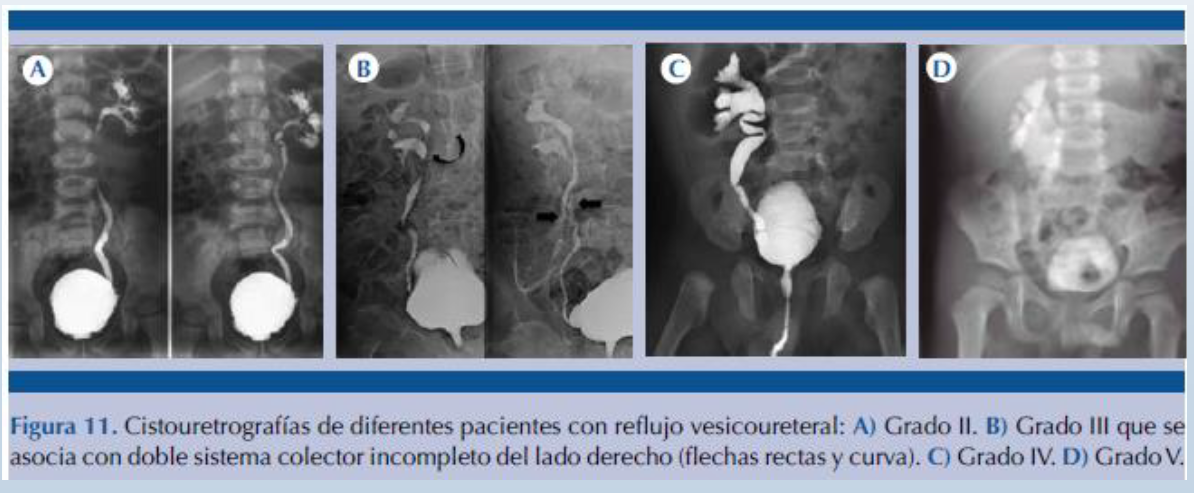
\includegraphics[width=1\linewidth]{imagenes/cisto reflujo.png}
    \caption{Reflujo vesicoureteral}
    \label{fig:c5}
\end{figure}

\subsection*{Fístulas del tracto genitourinario}

Comunicaciones anómalas entre la vejiga y estructuras adyacentes (vagina, recto, piel). Se evidencian con contraste en la proyección lateral durante la micción o en las oblicuas, como opacificación de estructuras ajenas al tracto urinario.

\begin{figure}[h]
    \centering
    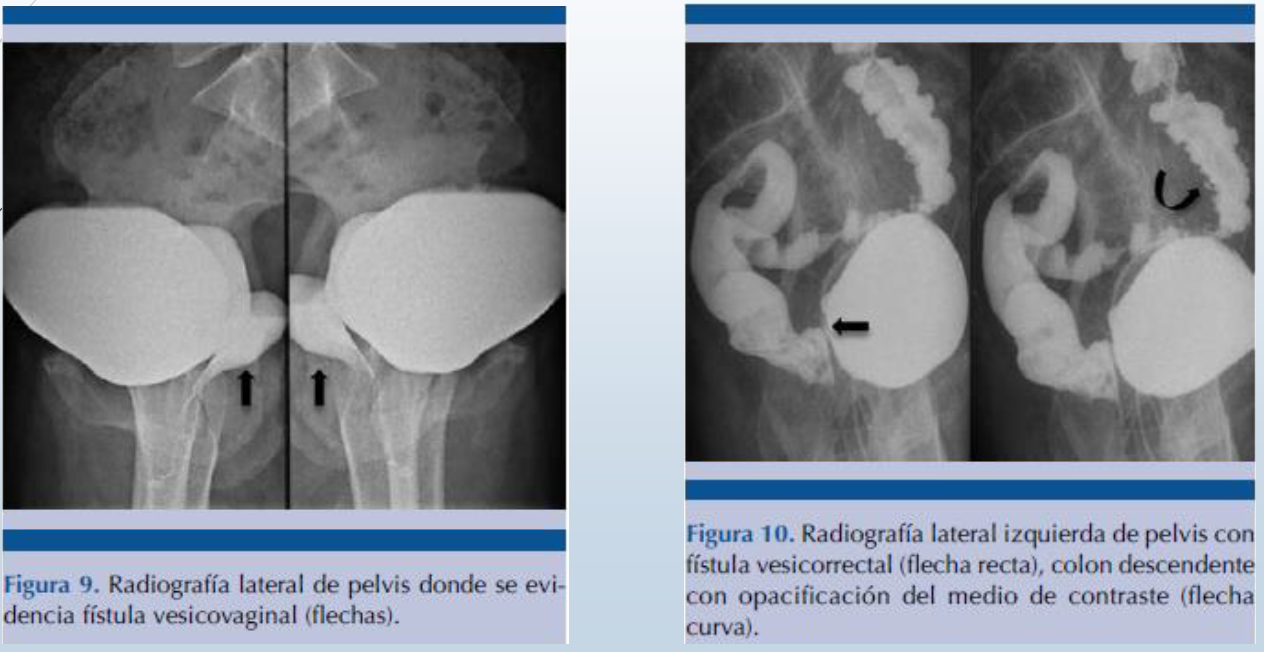
\includegraphics[width=1\linewidth]{imagenes/cisto fistulas.png}
    \caption{Fistulas}
    \label{fig:c6}
\end{figure}

\subsection*{Divertículo vesical}

Herniaciones de la mucosa vesical a través de la pared muscular de la vejiga. Aparecen como protrusiones saculares opacificadas con contraste adyacentes a la silueta vesical.

\begin{figure}
    \centering
    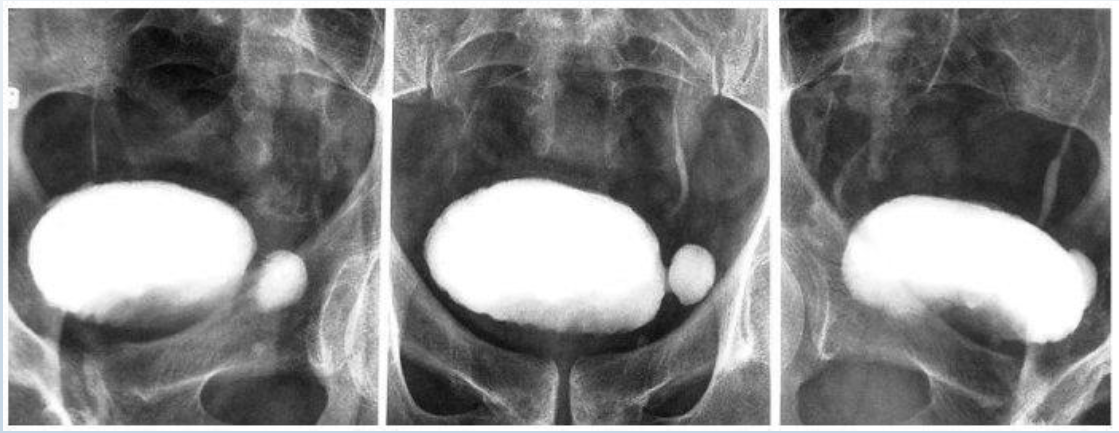
\includegraphics[width=1\linewidth]{imagenes/diverticulo.png}
    \caption{Diverticulo}
    \label{fig:c7}
\end{figure}

\subsection*{Cistocele e incontinencia urinaria}

Descenso de la vejiga con protrusión hacia la pared vaginal por debilidad del suelo pélvico. En la radiografía lateral (con maniobra de Valsalva o esfuerzo), la vejiga desciende por debajo del borde inferior de la sínfisis púbica. Se valoran los \textbf{ángulos uretrales} en la proyección lateral durante la micción.

\begin{figure}[h]
    \centering
    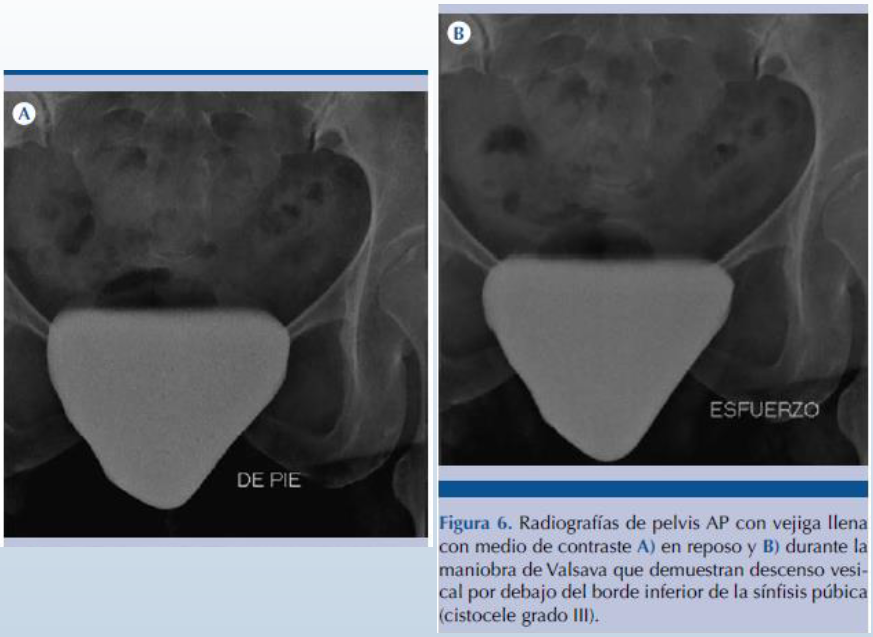
\includegraphics[width=1\linewidth]{cistocele.png}
    \caption{Cistocele}
    \label{fig:c8}
\end{figure}

\clearpage

% ============================================================
%  CIERRE --- ESQUEMA MENTAL FINAL
% ============================================================
\section*{Esquema Mental --- Repaso Final}

\begin{cajakeypoints}
\begin{center}
\textbf{\color{azulprincipal}
  Urocultivo negativo (72 h) $\rightarrow$ Sonda Foley $\rightarrow$ Contraste 400--450 mL $\rightarrow$ Serie de proyecciones $\rightarrow$ Post-miccional}\\[0.4em]
\textbf{\color{naranjadestacado}
  Residuo post-miccional $>$ 30\% = anormal. Estenosis anterior: llenado. Estenosis posterior: transmiccional.}\\[0.3em]
Uretra femenina: 4 cm \quad Uretra masculina: 17,5--20 cm \quad Sonda adulto: 12--18 F \quad Balón en hombre: 1--1,5 mL\\[0.3em]
\textbf{Protocolo:} simple $\to$ llenado AP $\to$ vejiga llena AP/oblicuas $\to$ miccional lateral $\to$ post-miccional
\end{center}
\end{cajakeypoints}

\vspace{1em}
\hrule
\vspace{0.5em}
{\footnotesize \textit{Fuente: material de clase --- Imagenología Especializada I, UdelaR 2026. Lic. Camila Mier.}}